\subsection{Code Performance and Workflow}

%\begin{SCtable}[1.]
%  \centering % center the table
%  \begin{tabular}{crrr} % alignment of each column data
%    \toprule
%    $V$ & $N$ & $t/s$ per solve & speedup\\
%    \midrule
%    $64^3\times128$ & 8 & 3.60 & 1\\
%    & 16 & 2.04 & 1.76\\
%    \midrule
%    $80^3\times160$ & 20 & 2.75  & 1\\
%    & 40 & 1.59 & 1.72\\
%    \bottomrule
%  \end{tabular}
%  \caption{Timings for QUDA MG solves on NVIDIA's Selene supercomputer
%  for one configuration of ensemble cB211.072.64 and one of ensemble
%  cC211.06.80 with $N$ the number of GPUs.}
%  \label{tab:MGsolver}
%\end{SCtable}


%All performance results have been measured on JUWELS Booster
About 90\% of the total run-time in the different parts of our research proposal is spent in QUDA's MG solver, the scaling behavior of which depends on the performance of the fine-grid Dirac operator ($D$) in double and single precision, as well as the intermediate-grid ($D_c$) and coarse-grid ($D_{cc}$) Dirac operators in half precision, which all have slightly different scaling behaviors due to the amount of parallelism that can be exposed on each grid.
On many nodes, only a small part of the solver time is spent in other kernels such as linear algebra.
Because the MG algorithm has substantial device memory requirements, it cannot be run as a whole on few GPUs and then scaled to many GPUs.
Similarly, it cannot be weak-scaled using synthetic data as the amount of time spent in each kernel depends on the physical properties of the Dirac operator to be inverted (and the associated gauge field).
Therefore, we demonstrate scalability via
\begin{itemize}
	\item  a combination of micro-benchmarks of the individual kernels depicted in \Cref{fig:quda_dirac_strong},
	\item time-to-solution of the multigrid solver in \Cref{tab:MGsolver},
	\item and a comparison of the time-to-solution obtained on various HPC systems equipped with NVIDIA GPUs  in \Cref{fig:multigrid_comparison}.
\end{itemize}
As depicted in \Cref{fig:quda_dirac_strong}, the scaling of the kernels involving the full-sized problem is close ideal up to a large number of nodes.
Only the coarse-grid Dirac operators, $D_c$ and $D_{cc}$, do not show a good scaling due to the significantly reduced problem size.
The multigrid solver is the only component affected by it and its scaling is sub-optimal due to the fact that most of the time is spent on the coarse-grid kernels. For this reason we use in our calculations the smallest number of nodes where our full problem can fit and run in parallel multiple jobs on different configurations.
The nodes we will used are reported in Table~\ref{tab:MGsolver}, respect to the
previous stage of this project we manage to optimize the memory footprint
of our run such that we can run in half of the nodes for the ensembles cB211.072.64
and cC211.06.80 resulting in more efficient runs.
In our runs the majority of the time will be spend in the setup of the MG
which will only be necessary for the first inversion for each values of the momentum.
%We will use 8 nodes for the cB211.072.64 ensemble, 24 nodes for the  , 20 nodes for the cC211.06.90 ensemble
%and 96 for the cD211.054.96 ensemble.

\begin{SCfigure}[0.5]
	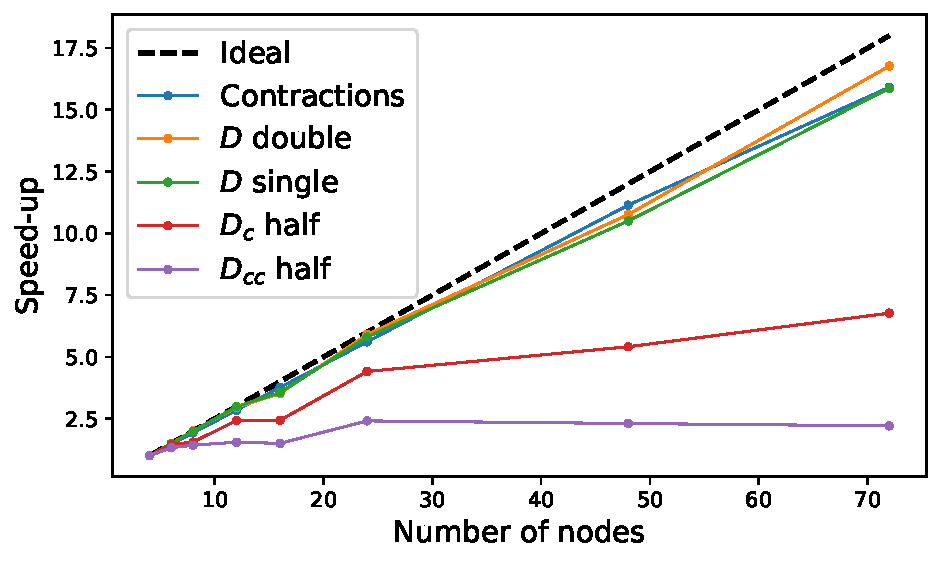
\includegraphics[width=0.6\textwidth]{plots/speedup.pdf}
	\caption{Strong scaling study of the contraction kernels and the QUDA Dirac operators on the fine ($D$), intermediate ($D_c$) and coarse ($D_{cc}$) grids for the cD211.054.96 having a lattice of size $96^3\times128$.}
	\label{fig:quda_dirac_strong}
\end{SCfigure}

\begin{table}%[1.]
	\centering % center the table
	\begin{tabular}{cccccccc} % alignment of each column data
		\toprule
		Ensemble      & $V$             & $N$ & $t/s$ MG setup & $t/s$ MG update & \multicolumn{3}{c}{$t/s$ MG inversion}                         \\
		              &                 &     &                &                 & $\ell$-quark                           & $s$-quark & $h$-quark \\
		%		\midrule
		\midrule
		% cAp211.077.64 & $64^3\times128$ & 8  & 52.6 & 0.5  & 2.6  & 0.8 & 0.3\\
		\midrule
		cB211.072.48  & $48^3\times96$  & 2   & 35.7           & 0.7             & 0.7                                    & 0.9       & 0.7       \\
		cB211.072.64  & $64^3\times128$ & 4   & 87.5           & 0.9             & 3.3                                    & 1.3       & 1.0       \\
		% cB211.072.64  & $64^3\times128$ & 8   & 51.5           & 0.5             & 2.6                                    & 0.8       & 0.3       \\
		cB211.072.96  & $96^3\times192$ & 24  & 57.9           & 1.0             & 4.15                                   & 1.1       & 1.1       \\
		\midrule
		% cC211.06.80   & $80^3\times160$ & 20  & 36.5           & 0.6             & 1.9                                    & 0.8       & 0.8       \\
		cC211.06.80   & $80^3\times160$ & 10  & 62.9           & 1.0             & 2.7                                    & 1.1       & 1.2       \\
		%		\midrule
		% cC211.06.112 & $112^3\times224$ & 56 & 43.6 & 0.9 & 2.87 & 1.0 & 0.5 \\
		\midrule
		cD211.054.96  & $96^3\times192$ & 24  & 46.0           & 1.0             & 2.5                                    & 1.0       & 1.2       \\
		\midrule
		cE211.044.112 & $112\times224$  & 56  & 43.6           & 1.0             & 2.87                                   & 1.0       & 1.3      \\
		\bottomrule   &
	\end{tabular}
	\caption{Timings for QUDA solves the ensembles we will use in this project.
		The light ($\ell$) and strange ($s$) quarks are inverted using the MG solver.
		The heavy ($h$) quark is inverted using the CG solver.
	}
	\label{tab:MGsolver}
\end{table}

\begin{SCfigure}[0.5]
	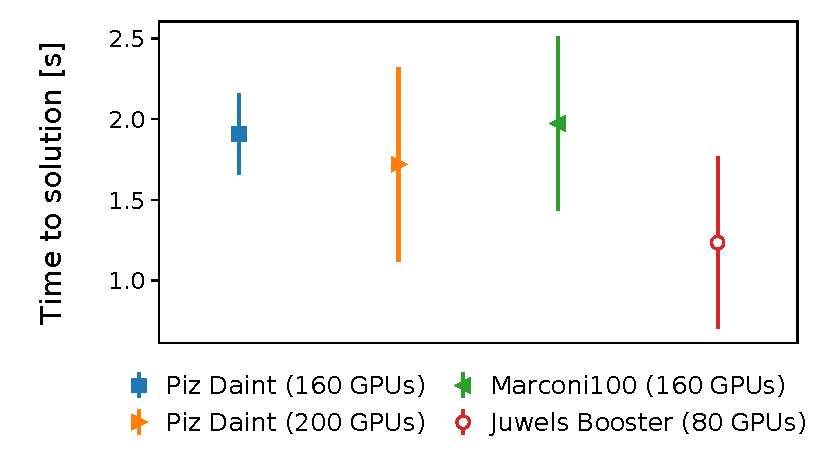
\includegraphics[width=0.6\textwidth]{plots/comparison.pdf}
	\caption{Comparison of the time to solution of the multigrid solver for the cC211.06.80 ensemble on different HPC systems in Europe and number of nodes.}
	\label{fig:multigrid_comparison}
\end{SCfigure}

Furthermore, in \Cref{fig:multigrid_comparison} we show a comparison of the time-to-solution for the cC211.06.80 ensemble measured on various
HPC systems in Europe equipped with different models of NVIDIA GPUs. We show results obtained on Piz Daint at CSCS equipped with P100, on Marconi100 at Cineca equipped with V100 and on the JUWELS Booster equipped with A100. The latter shows a time-to-solution about 40\% than the other systems using half of the GPUs. This is thanks to the improved performance of the latest model but also thanks to the significantly larger device memory available. Therefore our application has a significant speed-up on the GPU architecture offered by the JUWELS Booster.


\endinput
